\documentclass[10pt, a5paper]{article}
\usepackage{pdfpages}
\usepackage{parallel}
\usepackage[T2A]{fontenc}
\usepackage{ucs}
\usepackage[utf8x]{inputenc}
\usepackage[polish,english,russian]{babel}
\usepackage{hyperref}
\usepackage{rotating}
\usepackage[inner=2cm,top=1.8cm,outer=2cm,bottom=2.3cm,nohead]{geometry}
\usepackage{listings}
\usepackage{graphicx}
\usepackage{wrapfig}
\usepackage{longtable}
\usepackage{indentfirst}
\usepackage{array}
\newcolumntype{P}[1]{>{\raggedright\arraybackslash}p{#1}}
\frenchspacing
\usepackage{fixltx2e} %text sub- and superscripts
\usepackage{icomma} % коскі ў матэматычным рэжыме
\PreloadUnicodePage{4}

\newcommand{\longpage}{\enlargethispage{\baselineskip}}
\newcommand{\shortpage}{\enlargethispage{-\baselineskip}}

\def\switchlang#1{\expandafter\csname switchlang#1\endcsname}
\def\switchlangbe{
\let\saverefname=\refname%
\def\refname{Літаратура}%
\def\figurename{Іл.}%
}
\def\switchlangen{
\let\saverefname=\refname%
\def\refname{References}%
\def\figurename{Fig.}%
}
\def\switchlangru{
\let\saverefname=\refname%
\let\savefigurename=\figurename%
\def\refname{Литература}%
\def\figurename{Рис.}%
}

\hyphenation{admi-ni-stra-tive}
\hyphenation{ex-pe-ri-ence}
\hyphenation{fle-xi-bi-li-ty}
\hyphenation{Py-thon}
\hyphenation{ma-the-ma-ti-cal}
\hyphenation{re-ported}
\hyphenation{imp-le-menta-tions}
\hyphenation{pro-vides}
\hyphenation{en-gi-neering}
\hyphenation{com-pa-ti-bi-li-ty}
\hyphenation{im-pos-sible}
\hyphenation{desk-top}
\hyphenation{elec-tro-nic}
\hyphenation{com-pa-ny}
\hyphenation{de-ve-lop-ment}
\hyphenation{de-ve-loping}
\hyphenation{de-ve-lop}
\hyphenation{da-ta-ba-se}
\hyphenation{plat-forms}
\hyphenation{or-ga-ni-za-tion}
\hyphenation{pro-gramming}
\hyphenation{in-stru-ments}
\hyphenation{Li-nux}
\hyphenation{sour-ce}
\hyphenation{en-vi-ron-ment}
\hyphenation{Te-le-pathy}
\hyphenation{Li-nux-ov-ka}
\hyphenation{Open-BSD}
\hyphenation{Free-BSD}
\hyphenation{men-ti-on-ed}
\hyphenation{app-li-ca-tion}

\def\progref!#1!{\texttt{#1}}
\renewcommand{\arraystretch}{2} %Іначай формулы ў матрыцы зліпаюцца з лініямі
\usepackage{array}

\def\interview #1 (#2), #3, #4, #5\par{

\section[#1, #3, #4]{#1 -- #3, #4}
\def\qname{LVEE}
\def\aname{#1}
\def\q ##1\par{{\noindent \bf \qname: ##1 }\par}
\def\a{{\noindent \bf \aname: } \def\qname{L}\def\aname{#2}}
}

\def\interview* #1 (#2), #3, #4, #5\par{

\section*{#1\\{\small\rm #3, #4. #5}}

\def\qname{LVEE}
\def\aname{#1}
\def\q ##1\par{{\noindent \bf \qname: ##1 }\par}
\def\a{{\noindent \bf \aname: } \def\qname{L}\def\aname{#2}}
}

\begin{document}
\title{Голос спонсора: SaM Solutions}
%\author{}
\date{}
\maketitle

Компания SaM Solutions выступает в роли системо-образующего спонсора конференции Linux Vacation Eastern Europe, с момента зарождения LVEE в 2005 году и на протяжении всех лет её проведения. 

Сложившаяся корпоративная практика не случайна. Продукты и решения, задействующие Linux и другие Free/Open Source Software проекты, составляют заметную часть пакета разработок SaM Solutions. Кадровая политика компании направлена на поощрение профессионального развития своих сотрудников, организацию их эффективного отдыха и привлечение хорошо мотивированных кандидатов к работе на компанию. Формат конференции LVEE успешно позволяет решать все три задачи. 

Одним из направлений нашей деятельности является направление Linux/Unix разработок. Специалисты компании на протяжении десятилетий работают с СПО. Компанией реализован ряд проектов по адаптации ОС GNU/Linux для работы в различных устройствах, построенных на таких платформах как ARM, PowerPC, x86, MIPS. В последние годы "--- на ведущие позиции выходит разработка управляющего ПО для серверов Enterprise-класса, от низкоуровнего BMC Firmware на основе Linux до высокоуровневых систем контроля виртуализации и графических интерфейсов управления. Надёжность, качество и широкий функционал множества свободных проектов позволяет строить нам системы любого уровня и сложности, опираясь на высококачественные готовые компоненты.

Мы разрабатываем, модифицируем и адаптируем различное свободное програмное обеспечение для наших заказчиков, но не забываем о нём и для своих собственных нужд "--- наши сотрудники используют в своей работе существующие програмные продукты и вносят вклад в их развитие. Часть внутренней инфраструктуры, а именно интранет-сеть компании, тестовые стенды отдела контроля качества, рабочие места сотрудников профильных подразделений "--- также работает под управлением СПО (серверные и десктопные платформы GNU/Linux и FreeBSD).

По указанным причинам компания заинтересована в развитии движения open source, в продвижении свободных программных продуктов, и участие в конференции разработчиков и пользователей СПО.

В рамках Unix/Linux направления успешно выполнены проекты для таких знаковых заказчиков, как  Novell/SUSE, Fujitsu Technology Solutions  и осуществляется партнёрство с компаниями IBM и \linebreak Oracle/Sun в области Open Source решений.

Линукс-отдел компании SaM Solutions (Dept6/DDC3) уже более десяти лет является настоящей неофициальной кузницей кадров для специалистов в области Free/Open Source Software (FOSS). Код наших сотрудников есть в таких известных свободных проектах как Linux Kernel, Debian GNU/Linux, Alt Linux, Samba, wxWidgets, языке Ruby и его библиотеках и многих других. И SaM Solutions продолжает двигаться вперёд, не останавливаясь на достигнутом.
\begin{figure}[ht]
\centering{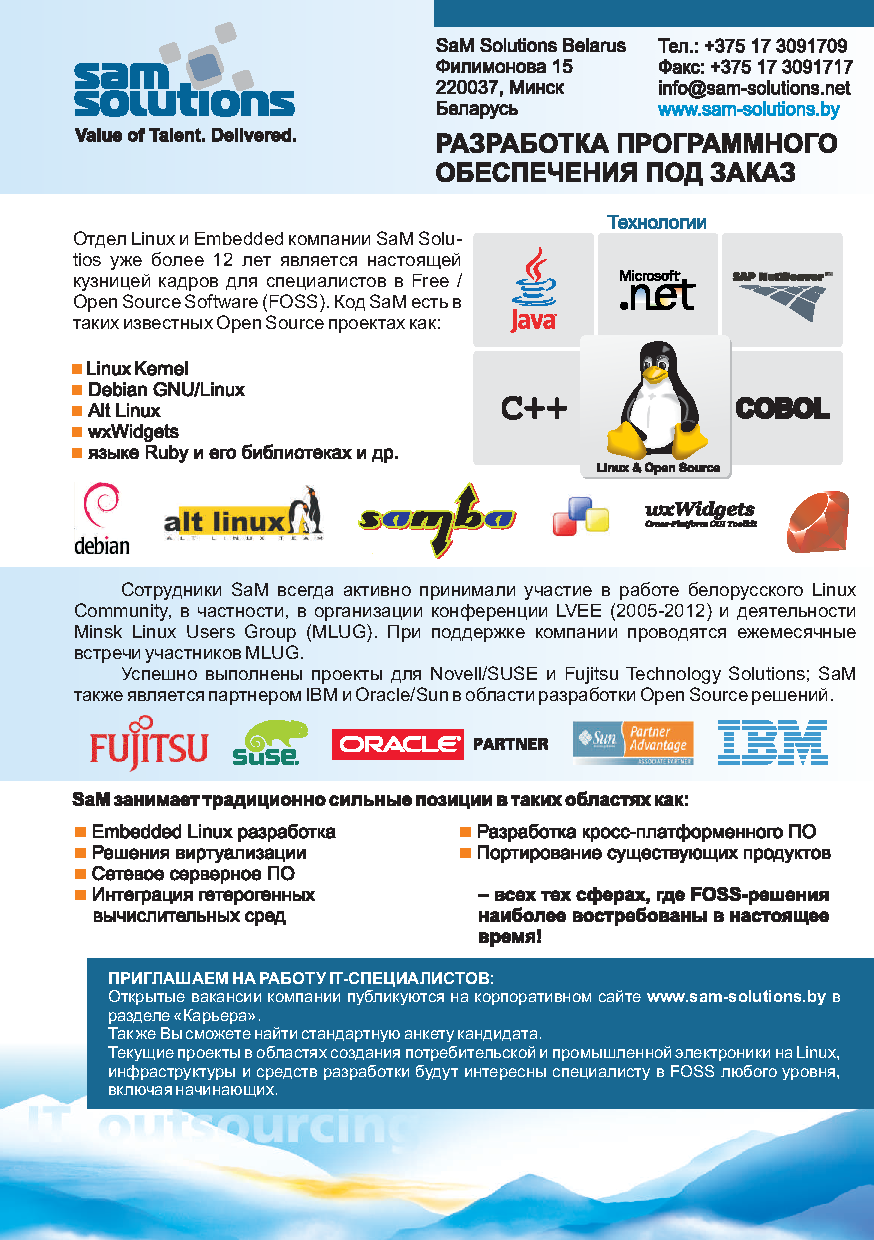
\includegraphics[height=11.8cm]{48_spons_sams.pdf}}
\end{figure}
\end{document}


